% Metódy inžinierskej práce

\documentclass[10pt,a4paper]{article}
\usepackage[english]{babel}%\ the laguage for this article is english
%\usepackage[T1]{fontenc}
\usepackage[IL2]{fontenc} % better typesetting of the letter L than in T1
\usepackage[utf8]{inputenc}
\usepackage{graphicx}
\graphicspath{{./}}%\ path for picture
\usepackage{url} % \url command to format URLs
\usepackage{hyperref} % linke to text
\usepackage{cite}

\pagestyle{headings}

\title{Mobile Games} %\It is the title of my article.

\author{Nematullah Hasani\\[1pt]
	{\small Slovak Technical University in Bratislava}\\
	{\small Faculty of Informatics and Information Technologies}\\
	{\small \texttt{xhasani@stuba.sk}}
	}

\date{\small 6. november 2022} % edit

\begin{document}
\maketitle

\begin{abstract}

Due to the advancement of technology and the increase in the model and quality of mobile phones, we are witnessing the growth of mobile games. Currently, there are many mobile games in the mobile software stores and Play Store and these games are increasing. This has caused customers to get confused while shopping. In this article, I tried to introduce you to the history of mobile games, which were the first mobile games? I am still trying to introduce different types of mobile games, what are their advantages and disadvantages. By reading this article, you will also get to know the most famous mobile games of the day.
\end{abstract}



\section{Introduction}

With the rapid growth of mobile phone technology, services and the important role of mobile phone in human life can be seen. Mobile games are one of the most exciting things you can play in your free time, which formed a small part of the game world in the beginning, but now they are one of the most important types of digital entertainment. For this reason, in this article I will deal specifically with mobile games. Looking at the history of mobile games, what were the first mobile games? What are the types of mobile games and the most important mobile games today? And you will also get to know the most famous organizations that make mobile games. In addition to this content, you will know what are the advantages and disadvantages of mobile games. By reading this article, you will get information about these contents.

\section{Mobile games}%\the main part of article.
Since smartphones have become a part of people's lives~\cite{liang2011effect}, there is a good opportunity for various game companies to provide their ideas and games to users. Mobile games are not a new phenomenon that we have encountered recently with their expansion. There are different types of mobile devices, but the way mobile games are placed on the mobile phone is divided into two separate parts~\cite{mayra2015mobile}, which are the pre-installed games and the other are the games that are available in the Play Store or Game-net. which is provided to us by purchase or installation. In the next part, I will discuss the history of mobile games, it has been a long time since the release of various mobile games, and with the increase in the number of users, Android can be considered as an independent game platform.

Every year, many games in different styles are released in the market, which have special and unique capabilities and features. Game platforms and consoles also have a high variety, and mobile phones can be considered one of the most popular game platforms.


\section{History of mobile games} \label{history mobile games}%\A brief overview of the history of mobile games
The early history of mobile games does not begin with the introduction of the first handheld electronic game in the late 1970s. Although the evolution and improvement in handheld electronic games were seen in this decade, these things did not apply to mobile games.

The era of mobile gaming began in 1994 with the game~\textit{\textbf{Tetris}} on the Hagenuk MT-2000. 3 years later in 1997,~\cite{mayra2015mobile} Nokia introduced one of the most popular mobile games called ~\textit{\textbf{Snake}}, which was pre-installed on Nokia phones. This game, which was on more than 400 million devices worldwide, is also known as the first two-player mobile game in history.

\begin{figure}[h]%\This image is from the first mobile game.
    \centering
    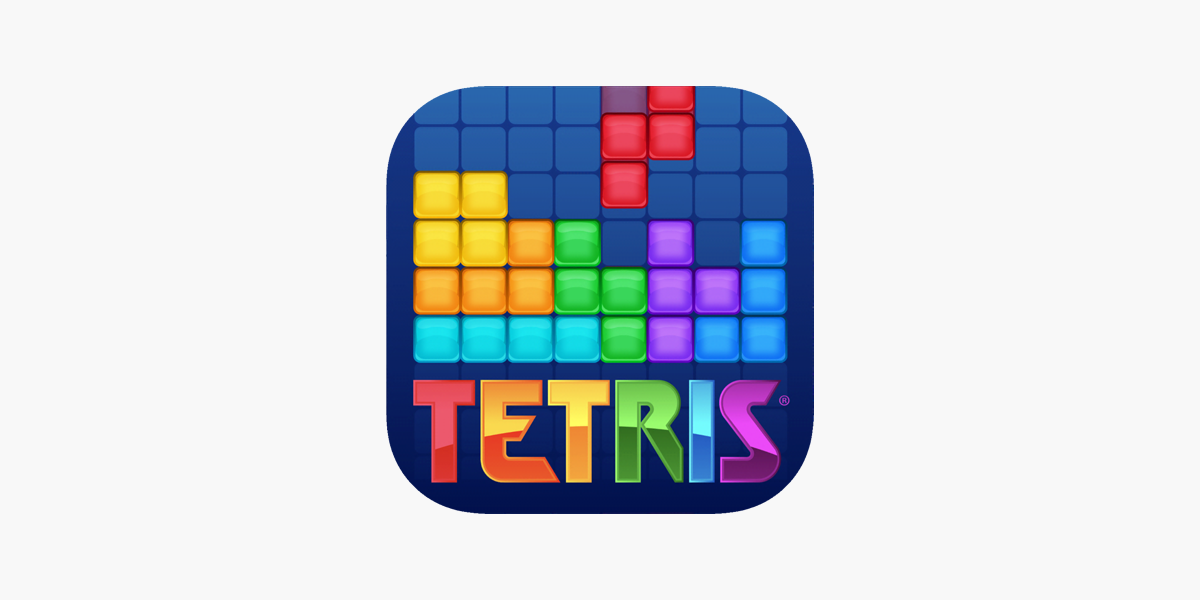
\includegraphics[width=.6\textwidth]{Tetris.png}
    \caption{It is the  sample of first mobile game called \textit{Tetris}}
    \label{fig:Tetris}
\end{figure}

2000 was associated with the introduction of the first downloadable game and 2008 with the opening of the first virtual store providing mobile content by Apple.

\section{Types of mobile games}%\In this section, I categorized mobile games
There are many different types of mobile games, and they are usually categorized by their main features or goals – not by the type of gameplay they have.
Game categories can also have subcategories, and many games fall into multiple categories.~\cite{idtech}
\begin{table}[h]
\textbf{Mobile games categories}\\ 
\begin{tabular}{|c |c |c| }
 \hline\hline
  \textbf{Action games} & \textbf{Action-adventure games} & \textbf{Adventure games} \\ 
  \hline
 \textbf{Role-playing games} & \textbf{Simulation games} & \textbf{Strategy games} \\
 \hline
 \textbf{Sports games} &\textbf{ Puzzle games} & \textbf{Idle games} \\
 \hline
\end{tabular}
\caption{It shows the categories of mobile games.}
\label{table:1}
\end{table}
\section{Advantage of mobile games}%\I have explained the advantages of mobile games in a list here.
Until today, mobile games are known as one of the most entertaining pastimes possible. Although researchers have published reviews and opinions about the negative effects of these games. Here we have an overview of the benefits of mobile games, which, in addition to being fun, make your brain and memory grow and strengthen.~\cite{azbigmedia}

\begin{itemize}
    \item \textbf{Strengthens problem solving skills:}
       The majority of mobile games develop brain power, which gives players creativity to solve problems and the ability to think more.
    \item\textbf{It allows for moments to recharge:}
    It's not new that taking a moment away from our work to think about something else makes our brains recharge and focus more on solutions.
    \item\textbf{It  increases the efficiency of creativity:}When playing mobile games, the player tries to play creatively and control time more.
    \item\textbf{It improves morale and team building:}Weekend breaks are enjoyable for everyone because they are away from the work area and their brains are not busy. Mobile games also allow you to relax and increase the ability to work as a team in important projects.
    \item\textbf{It reduces stress:}The best and most important reason that gaming can be beneficial to players is that it gives employees a healthy way to relieve stress. During the game, you will be in different scenes that will help reduce your stress. Another thing is that you will not have more free time to turn to drugs.
\end{itemize}

 \section{Disadvantage of mobile games}%\I have explained the disadvantages of mobile games in a list here.
every thing has its benefits and damage until you got information about the advantage of mobile games it is time to review the disadvantage of mobile games.
\begin{itemize}
    \item \textbf{Weakness in vision:} More attention and thinking is required during to play game, this makes the player not blink at all in a minute, this itself is considered a negative effect, it causes poor eyesight.
    \item\textbf{Increasing the probability of disease:} Continuous use of mobile phones causes the emergence of various diseases in humans over time. In this sense, be cautious in using mobile games. Every electronic device emits radiation that cannot be seen.
    \item\textbf{Reduction of social relations:} The more people have contact with the outside environment, the more social relationships they have. People who play alone have weak social relationships.
Mobile games are mostly played alone, so it keeps people isolated and away from society.
Being isolated and reducing the level of communication is one of the disadvantages of playing mobile games for people, which should be taken seriously. Because this issue may affect his future.
\end{itemize}

\bibliography{bibliography.bib}
\bibliographystyle{siam} 
\end{document}
